\documentclass[convert]{standalone}

\usepackage{tikz}
\pagestyle{empty}

% INT_AY20_MP3_L22_Fig01_Bar_magnet_w_field.tex

\begin{document}
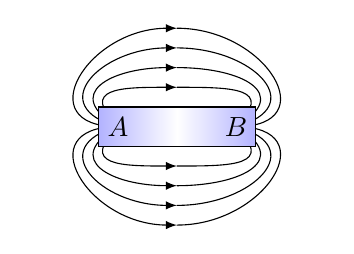
\begin{tikzpicture}[> = latex, scale = 0.5]
	
	% Magnetic field lines
	
	\begin{scope}[->]
	
		\draw (-1.5, 0) to [out = 135, in = 180, looseness = 2] (0, 1);
		\draw (-1.5, 0) to [out = 150, in = 180, looseness = 2] (0, 1.5);
		\draw (-1.5, 0) to [out = 165, in = 180, looseness = 2] (0, 2);
		\draw (-1.5, 0) to [out = 180, in = 180, looseness = 2] (0, 2.5);
	
		\draw (-1.5, 0) to [out = -135, in = 180, looseness = 2] (0, -1);
		\draw (-1.5, 0) to [out = -150, in = 180, looseness = 2] (0, -1.5);
		\draw (-1.5, 0) to [out = -165, in = 180, looseness = 2] (0, -2);
		\draw (-1.5, 0) to [out = -180, in = 180, looseness = 2] (0, -2.5);
		
	\end{scope}
	
	\draw (0, 1) to [out = 0, in = 45, looseness = 2] (1.5, 0);
	\draw (0, 1.5) to [out = 0, in = 30, looseness = 2] (1.5, 0);
	\draw (0, 2) to [out = 0, in = 15, looseness = 2] (1.5, 0);
	\draw (0, 2.5) to [out = 0, in = 0, looseness = 2] (1.5, 0);
	
	\draw (0, -1) to [out = 0, in = -45, looseness = 2] (1.5, 0);
	\draw (0, -1.5) to [out = 0, in = -30, looseness = 2] (1.5, 0);
	\draw (0, -2) to [out = 0, in = -15, looseness = 2] (1.5, 0);
	\draw (0, -2.5) to [out = 0, in = 0, looseness = 2] (1.5, 0);

	% Bar magnet
	
	\draw [left color = blue!30, right color = blue!30, middle color = white] (-2, -0.5) rectangle (2, 0.5);
	\node at (-1.5, 0) {$A$};
	\node at (1.5, 0) {$B$};

\end{tikzpicture}
\end{document}